\begin{frame}{Riadená sústava}
\begin{itemize}
  \item<1-> Nestabilná \angl{unstable} - duh...
  \item<2-> Nelineárna \angl{nonlinear} - uhly, atď.
  \item<3-> \angl{underactuated} - 4 vstupy, 6 DOF výstup \citep{Douglas2018}
\end{itemize}
\begin{figure}
\centering
  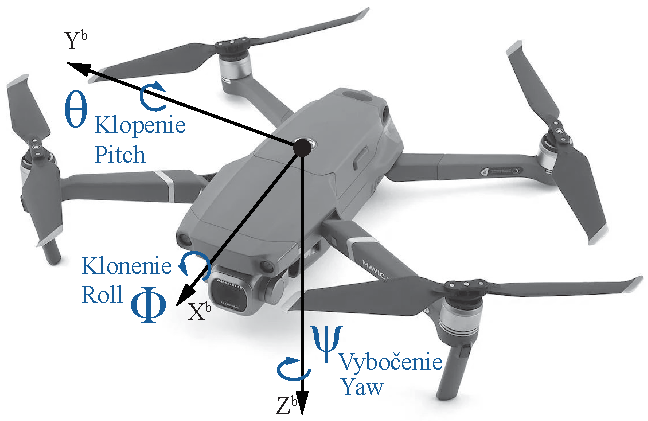
\includegraphics[width=\textwidth]{rollpitch}\\
\end{figure}
\end{frame}

\begin{frame}[t]{Rýchlosť zmeny uhlov}
\begin{itemize}
  \item<1-> Tvárme sa, že poznáme žiadanú uhlovú rýchlosť orientácie $r_{\dot{\Theta}}$, $r_{\dot{\Phi}}$ a $r_{\dot{\Psi}}$ resp $r_{\dot{h}}$ (vert. rýchlosť) a pre jednoduchosť sústredme len na rýchlosť zmeny klopenia ($\dot{\Theta}$).
  \item<2-> Sme na najnižšej úrovni, t.j. riadenie uhlovej rýchlosti \angl{rate controller} --- je to zároveň aj najdôležitejšia slučka, a máme 4 slučky \citep{AP:PID,PX4:PIDTuning}.
  \item<3-> Slučky sú nezávislé len pre malé uhly, lebo keď zvýšime letovú výšku $h$ pri väčších e.g. $\Theta$ tak zvýšime aj vertikálnu aj horizontálnu rýchlosť \citep{Douglas2018}!
  \item<4->  Je to aj najrýchlejšia slučka (cca. $f_s$=400--1000 Hz \citep{AP:PID,PX4:PIDTuning}) Meranie je komplexný problém sám v sebe, napr. low-pass gyro + notch \citep{Bresciani2020} alebo odhad
  \end{itemize}

  \begin{onlyenv}<1>
  \begin{figure}
\centering
  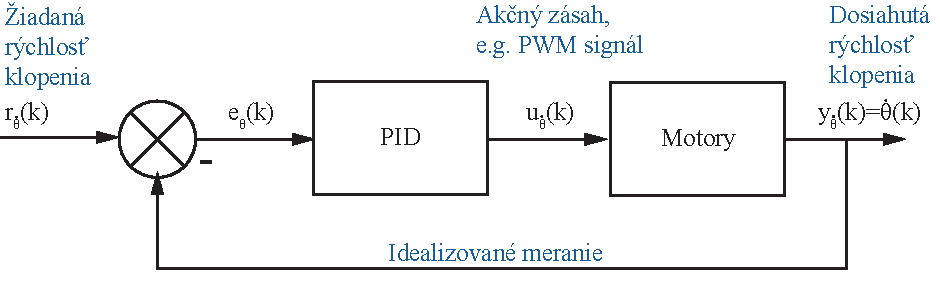
\includegraphics[width=\textwidth]{ATT_Rate}\\
\end{figure}
\end{onlyenv}

  \begin{onlyenv}<2-3>
  \begin{figure}
\centering
  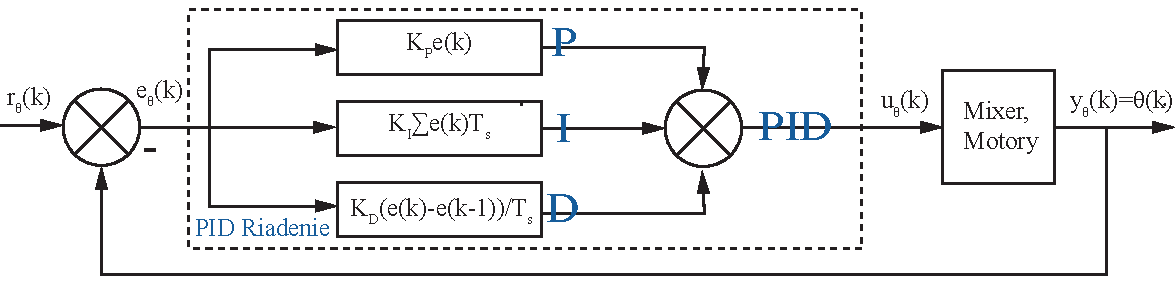
\includegraphics[width=\textwidth]{ATT_Rate2}\\
\end{figure}
\end{onlyenv}
  \end{frame}



  \begin{frame}{Pridelenie akčných zásahov}
  \begin{itemize}
    \item<1-> Aj keď slučky PID na tejto úrovni definujú žiadanú zmenu $u(k)$, musíme implementovať pridelenie riadenia \angl{control allocation} $u_M(k)$ (PWM, RC impulzy) do individuálnych motorov cez elektronické riadenie rýchlosti \angl{electronic speed control, ESC}.
     \item<2-> V najjednoduchšom prípade máme mapujeme pre každý motor 1-4 (alebo viac)
    \begin{align}
     u_{M1}(k) &= u_{\dot{h}}  + u_{\dot{\Phi}} + u_{\dot{\Theta}}  + u_{\dot{\Sigma}}\\
     u_{M2}(k) &= u_{\dot{h}}  - u_{\dot{\Phi}} + u_{\dot{\Theta}}  - u_{\dot{\Sigma}}\\
     u_{M3}(k) &= u_{\dot{h}}  + u_{\dot{\Phi}} - u_{\dot{\Theta}}  - u_{\dot{\Sigma}}\\
     u_{M4}(k) &= u_{\dot{h}}  - u_{\dot{\Phi}} - u_{\dot{\Theta}}  + u_{\dot{\Sigma}}
     \end{align}
\end{itemize}
    \begin{onlyenv}<1>
  \begin{figure}
\centering
  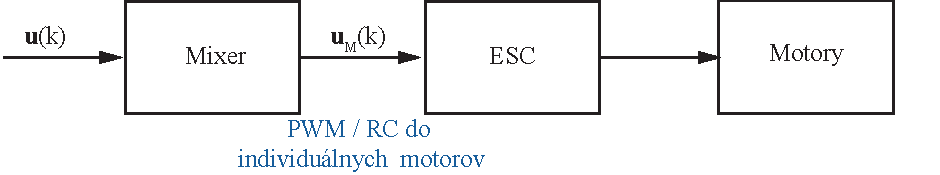
\includegraphics[height=20mm]{ATT_Allocation}\\
\end{figure}
\end{onlyenv}
    \begin{onlyenv}<2->
  \begin{figure}
\centering
  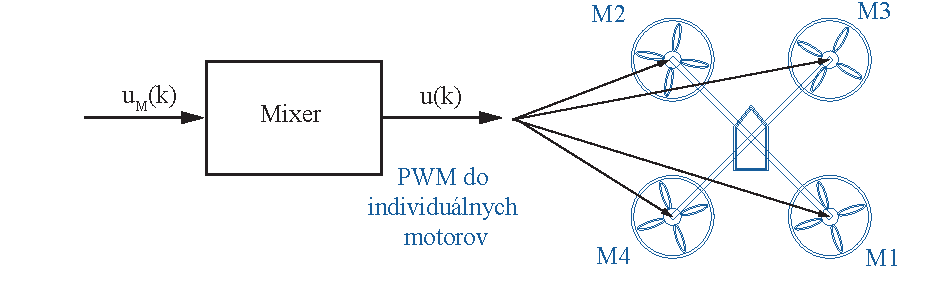
\includegraphics[height=20mm]{ATT_Allocation2}\\
\end{figure}
\end{onlyenv}
  \end{frame}

   \begin{frame}{Pridelenie akčných zásahov 2}
  \begin{itemize}
  \item<1->
        \begin{align}
     \begin{bmatrix}
       u_{M1}(k) \\
       u_{M2}(k) \\
       u_{M3}(k) \\
       u_{M4}(k)
     \end{bmatrix}=\underbrace{\begin{bmatrix}
                     +1 & +1 & +1 & +1 \\
                     +1 & -1 & +1 & -1 \\
                     +1 & +1 & -1 & -1 \\
                     +1 & -1 & -1 & +1
                   \end{bmatrix}}P =
                \begin{bmatrix}
                     u_{\dot{h}} \\
       u_{\dot{\Phi}} \\
       u_{\dot{\Theta}} \\
       u_{\dot{\Sigma}}
     \end{bmatrix}
     \end{align}

    \item<2-> Mapa $u_M(k)=Pu(k)$ kde $P$ matica pridelenia riadenia \angl{control allocation matrix}. Nemusí obsahovať iba jednotky, môže byť aj neštvorcová ale našťastie transformácia je stále lineárna \citep{Bresciani2020}.
    \item<3-> Môžeme priamo namapovať maticu efektivity akčných členov \angl{actuator effectiveness matrix} $B$, kde $P=B^{-1}$. Ak počet akčných zásahov = počtu akčných členov, používame inverziu ináč napr. Moore-Penroseovu pseudoinverziu $P=B^{\dagger}$ \citep{Bresciani2020}.
\end{itemize}
%    \begin{onlyenv}<1>
%  \begin{figure}
%\centering
%  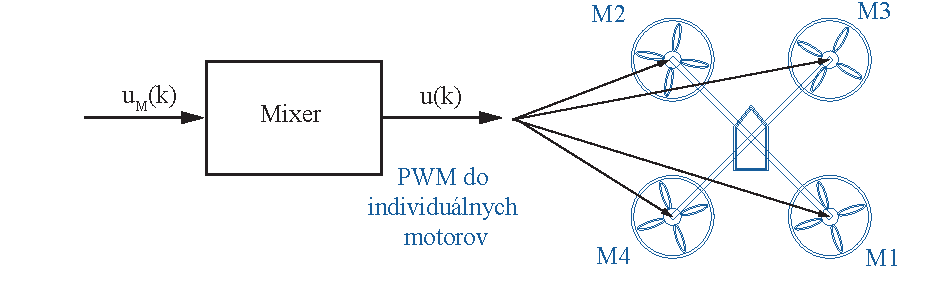
\includegraphics[width=\textwidth]{ATT_Allocation2}\\
%\end{figure}
%\end{onlyenv}
  \end{frame}



\begin{frame}[t]{Ohraničenie vstupov}
  \begin{itemize}
    \item<1-> Akčné zásahy majú svoje ohraničenia (\angl{constraints})
    \item<2-> Ako donútime ich dodržanie? Saturáciou (orezávaním) hodnôt, ktoré skutočne vypočíta PID.
    \item<3-> Saturácia vnáša nelinearitu, vplýva na výkon riadenia aj stabilitu.
    \item<4-> Aj iné veličiny môžeme saturovať, napr. žiadané hodnoty. Ako by sme ohraničili výstup?
  \end{itemize}

    \begin{onlyenv}<2->
  \begin{figure}
\centering
  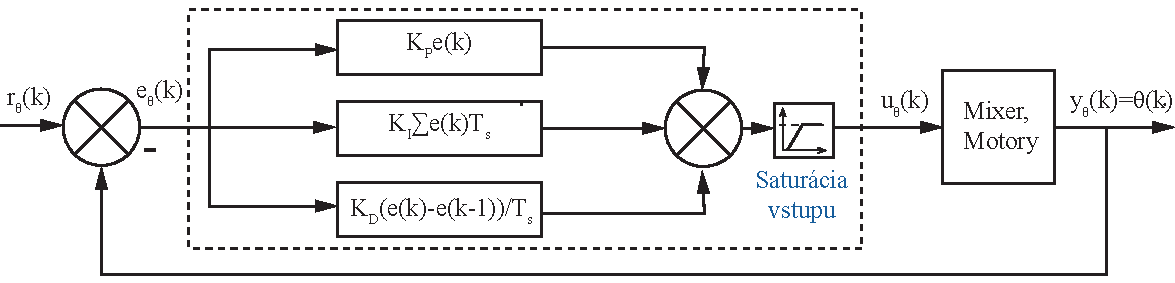
\includegraphics[width=\textwidth]{ATT_Rate3}\\
\end{figure}
\end{onlyenv}
\end{frame}


\begin{frame}[t]{Nahromadenie integračnej zložky}
  \begin{itemize}
    \item<1-> Integračná zložka ráta odchýlku v minulosti, preto ak akčné členy sú už na hraniciach možností - začína sa nahromaďovať \angl{windup}.
    %alebo sa to zbtočne nahromadí/začína sa zbytočne nahromaďovať (nemôže sa yačínať robiť sloveso v dokonavom vide...)
    \item<2-> Akonáhle sa vrátia akčné zásahy pod ohraničenia, nahromadená I zložka stále bude tlačiť systém na hranice možností, musí sa to chvíľu ``uvoľňovať'' \angl{unwind} a tým pádom prestrelíme \angl{overshoot} žiadané hodnoty
    \item<3-> To je saturácia integračnej zložky \angl{integral windup}.
    \item<4-> Môžeme používať rôzne triky, napr. ohraničiť veľkosť integračnej zložky, resp. vypnúť zložku pri určitých podmienkach.
  \end{itemize}
      \begin{onlyenv}<1-4>
  \begin{figure}
\centering
  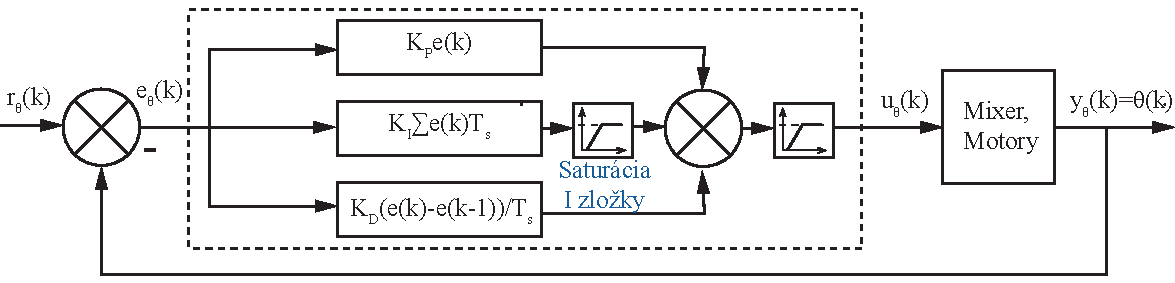
\includegraphics[width=\textwidth]{ATT_Rate4}\\
\end{figure}
\end{onlyenv}

      \begin{onlyenv}<5>
        \begin{itemize}
  \item<1-> ArduPilot - Ak akčný člen je akurát saturovaný, podrž hodnotu I zložky. Nižšie to môže ísť, vyššie nie \citep{AP:PID}.
  \item<2-> ArduPilot - Keďže máme kaskádnu konfiguráciu PID slučiek, saturačný znak postupuje cez hierarchiu nižšie a nižšie aby zastavil nahromadenie I zložky \citep{AP:PID}.
            \end{itemize}
      \end{onlyenv}

\end{frame}



\begin{frame}[t]{Šum a kopnutie derivačnej zložky}
  \begin{itemize}
    \item<1-2> Šum zo snímačov môže propagovať cez výpočet odchýlky riadenia do derivačnej zložky Vysokofrekvenčné zložky potom navýšia D zložku (čo je derivácia impulzu?)
    \item<2> Riešenie: Odchýlku riadenia pustíme cez dolnopriepustný \angl{low-pass} filter (LPF) --- Aj ArduCopter (20 Hz LPF) aj PX4 Autopilot používa \citep{AP:PID,PX4:PID}
    \item<3-> Náhle zmeny spôsobia ``kopnutie'' riadenia \angl{derivative kick}. (čo je derivácia impulzu?)
    \item<4-> Môžeme celkovo obísť zmenu žiadanej hodnoty a tým odchýlky  $e_\Theta(k)$ tak, že derivujeme výstup $y_\Theta(k)$\footnote{Riešenie v PX4, ArduCopter používa input shaping.}
  \end{itemize}
      \begin{onlyenv}<1-2>
  \begin{figure}
\centering
  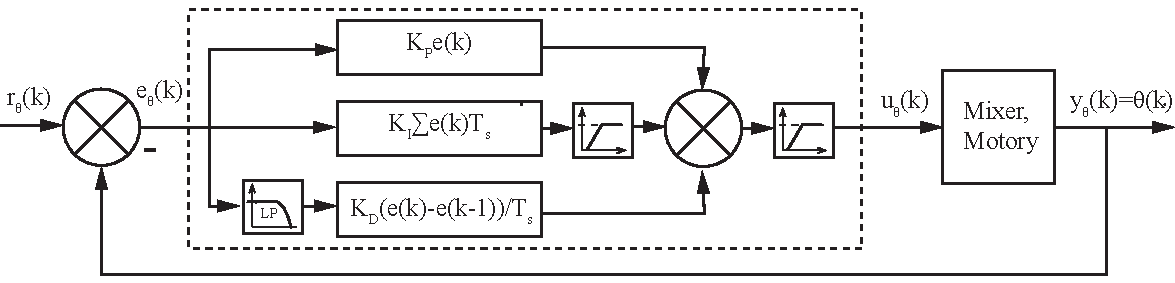
\includegraphics[width=\textwidth]{ATT_Rate5}\\
\end{figure}
\end{onlyenv}

\begin{onlyenv}<3->
  \begin{figure}
\centering
  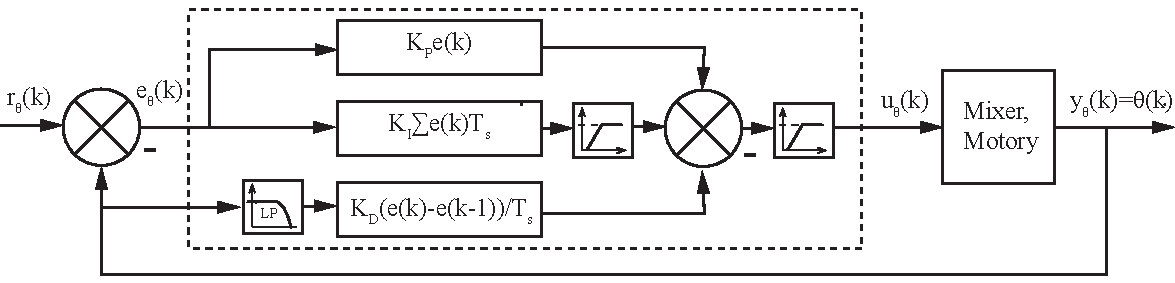
\includegraphics[width=\textwidth]{ATT_Rate6}\\
\end{figure}
\end{onlyenv}


\end{frame}

\begin{frame}{Ako to funguje v ``reálne''?}
\begin{onlyenv}<1>
  \begin{figure}
\centering
  \includegraphics[width=100mm]{PX4_Rate}\\
\end{figure}
\end{onlyenv}

\begin{onlyenv}<1>
  \begin{figure}
\centering
  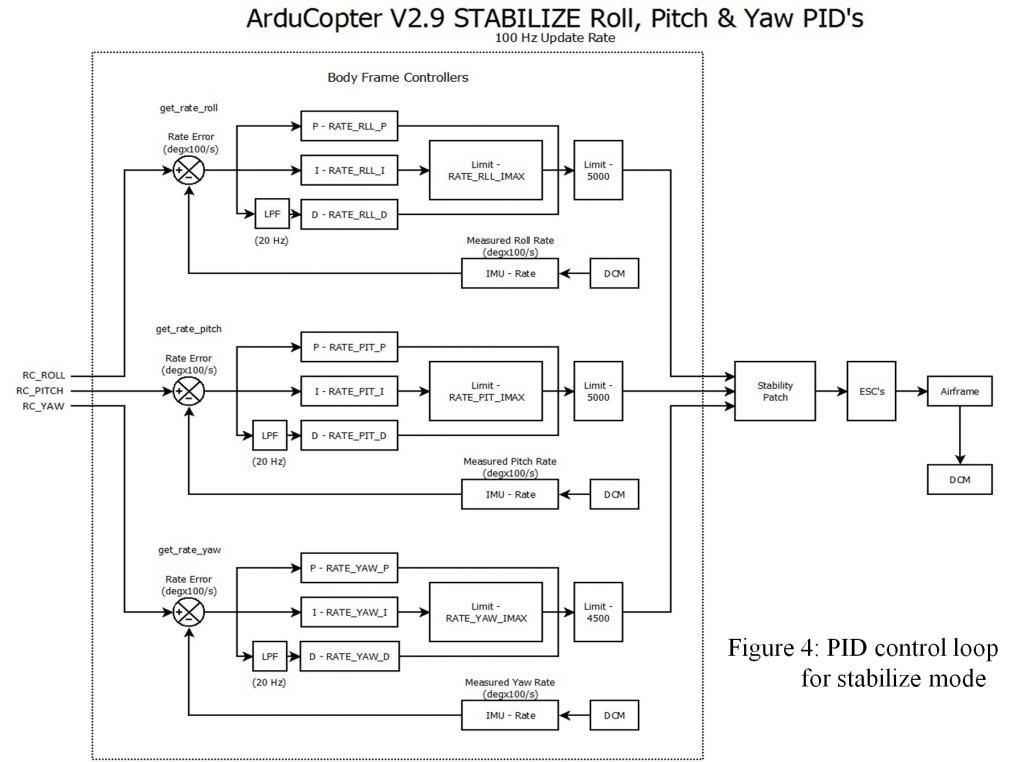
\includegraphics[width=100mm]{AP_Stabilize}\\
\end{figure}
\end{onlyenv}


\end{frame} 